%\documentclass{article}
\documentclass[a4paper,12pt]{article}
% Seitenränder in schön für Steven
\usepackage[paper=a4paper,left=25mm,right=25mm,top=25mm,bottom=25mm]{geometry}
\usepackage{enumitem}
\usepackage{amsmath}
\usepackage{float}
\usepackage{graphicx}
\usepackage{tikz}
\usepackage{titling}


% Schusterjungen und Hurenkinder bestrafen
\clubpenalty50000
\widowpenalty50000
\displaywidowpenalty=50000

% Buchstaben mit kringel drum: %
\newcommand*\mycirc[1]{%
	\begin{tikzpicture}[baseline=(C.base)]
	\node[draw,circle,inner sep=1pt](C) {#1};
	\end{tikzpicture}}

\newcommand*\red[1]{\textcolor{red}{#1}}

\author{Benedict Hans, Christoph Dollase, Steven Te\ss endorf}
\setlength{\droptitle}{-5em} % set the title to the top of the page

% ==========================
% ===== START HERE!! =======
% ==========================
\title{ \textbf{Problem Sheet 11}}
\setcounter{section}{11} % Nummer des Aufgabenblattes

\begin{document}	 
	\maketitle	 %Some Vodoo-magic
	
	\subsection{Network Components}
    \textbf{Discuss the function(-s) of the following network components: Repeater, hub, switch, bridge, router, 
    and gateway. Which "data" do they handle and on which layer of the ISO/OSI reference model do they operate?}
    \begin{itemize}[itemsep=0pt]
        \item \textbf{Repeater:} Receives signals and retransmits them. It operates on the physical layer.
        \item \textbf{Hub:} Receives a signal and splits it into multiple signals. After splitting it, it sends it
            to connected devices. It operates on the physical layer.
        \item \textbf{Switch:} Sends data to a target device after receiving them. Opens packets and searches for
            the target device. Operates on data link layer.
        \item \textbf{Bridge:} Transfers data packets between networks. A transparent bridge "knows" in which
            network devices are located. Operates on data link layer.
        \item \textbf{Router:} Opens packets and searches for the target network/device. Often used as gateway
            to different networks. Operates on Network Layer.
        \item \textbf{Gateway:} Connects to systems. Data can be edited. A Gateway can operate on all layers.
    \end{itemize}
	
	% Solution
	
	\subsection{Spanning Tree}
	\textbf{The spanning tree is an important connected graph of a computer network. On which layer of the ISO/OSI
    reference model is it created?} \newline
    The spanning tree is creates on basis of the Data Link Layer. \newline
    \newline

    \textbf{Why do we need to create a spanning tree? What is the important property?} \newline
    Two bridges connecting two LANs can get caught in a loop (due to a ring like structure) and continiously send
    data between each other without any party requiring it. A spanning tree can solve this problem. The tree 
    represents a clear hierarchy between the bridges and LANs with one root bridge. \newline
    \newpage

    \textbf{Create the spanning tree for the given network. The numbers at the edges specify the cost of each path
    ; the number in the vertices specify the switch ID.} \newline

    \begin{center}%h! sorgt dafür dass das Bild möglichst nicht woanders hingeschoben wird
	    %Erklärung: [width=0.5\linewidth] -> Bild ist maximal so breit wie die Hälfte des Schriftbildes
	    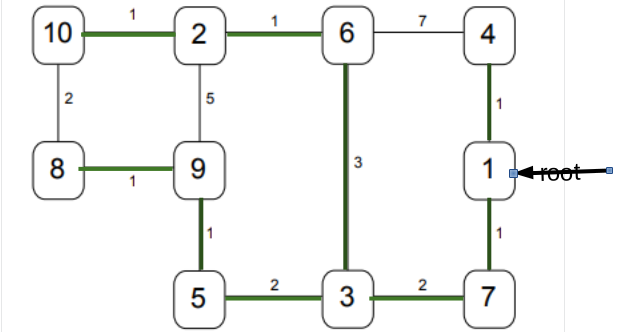
\includegraphics[width=0.5\linewidth]{tree.png} 
	    \caption{Spanning Tree}
    \end{center}
    	
\end{document}

% Hier nach passiert nichts mehr, daher nutzen wir das als kleines Cheat-Sheet ;)
% ===============================================================================

% Aufzählungen (auch merhstufig):
\begin{itemize}[itemsep=0pt]
	\item 
\end{itemize}

%Bilder eifnügen:
\begin{figure}[h!] %h! sorgt dafür dass das Bild möglichst nicht woanders hingeschoben wird
	%Erklärung: [width=0.5\linewidth] -> Bild ist maximal so breit wie die Hälfte des Schriftbildes
	\includegraphics[width=0.5\linewidth]{Bildname.jpg} 
	\caption{Bildunterschrift}
\end{figure}

%Tabelle einfügen:
\begin{table}[h!] %h! sorgt dafür dass die Tabelle möglichst nicht woanders hingeschoben wird
	\caption{Tabellenüberschrift}
	%hinter {tabular}: Anzahl Spalten (c=center, l=linksbündig, r=rechtsbündig, | Spaltenstriche)
	\begin{tabular}{|c|c|c} 
		A & B & C  \\ % \\ = return (neue zeile)
		\hline % horinzontale Linie
		0 & 1 & 2
	\end{tabular}
\end{table}
